%TC:ignore

To answer our research question, experiments were set up around the three components in the research question: climate, population and public health. 

The structural and parametric uncertainties resulted in five policies that will be tested. These policies were designed based on reality and are capable of providing a view of the policies' cost effectiveness and robustness. These policies will be discussed in Subsection \ref{s:environmentalfactors} to \ref{s:foodbehaviour}. 

We elaborate on the scenarios used to test these policies in Subsection~\ref{ch: detexp}.

%Policies in environment
\subsection{Environmental factors and policies to control disease vectors}
\label{s:environmentalfactors}
Two policies were implemented with regards to environmental factors and the biological disease vectors. Both are triggered by temperature, as this is the main driver of the population growth of flies, as explained in Section~\ref{fig:environmental_submodel}.

\subsubsection{Exposure control policy}
This policy decreases human exposure to infected flies: on the season when the disease vector is more prevalent, public campaigns will urge the population to keep organic waste properly closed and use fly nets \parencite{hald_use_2007}. Similar measures are used to prevent the spread of disease carrying mosquitoes in tropical countries \parencite{govella_why_2012}. %I know this for a fact because tropical country, but we might want to add a source.

The closed-loop policy is triggered by the temperature. If the temperature is above 20\degree c, the policy goes in effect. This temperature is based on the findings by \cite{schou_temperature_2013}. It assumes an immediate reduce of 20\% on the rate of human exposure to infectious flies. It was also assumed there would be an information delay of 2 weeks from the onset of the policy to full implementation.

\subsubsection{Fly population control policy}
When a certain threshold of fly population is reached, the government can initiate extermination campaigns to limit the spread of diseases. This can be generalised, or localised only around farms.

Likewise to the Exposure control policy, this policy is activated by temperature. Once the temperature gets above 20\degree c, the policy goes into effect. This immediately reduces the fly population to 80\%. We assume the effect is immediate, as this policy is not dependent on people's behaviour: the government can instantiate these immediately.

\iffalse
\begin{itemize}
    \item Public campaigns to prevent human exposure to infected flies: on the season when the disease vector is more prevalent, urge the population to keep organic waste properly closed and use fly nets \parencite{hald_use_2007}. Similar measures are used to prevent the reproduction of disease carrying mosquitoes in tropical countries. %I know this for a fact because tropical country, but we might want to add a source.
    \item Pest control measures: when a certain threshold of fly population is reached, the government can initiate extermination campaigns to limit the spread of diseases. This can be generalised, or localised only around farms.
%install pest control measures, including variables such as: intensity of extermination / frequency
%install threshold fly population value that activates pest control. The aim is to counteract effects of population growth to infected flies and infection rates.
%Note: could we connect fly population or proportion of infected flies to exposure rate??
\end{itemize}
\fi


\subsection{Food safety behaviours and policies}
\label{s:foodbehaviour}
With regards to food safety behaviours and policies, we looked at two insertion points in the chicken production cycle: the hygiene of the slaughtering process and the way food is handled from the slaughterhouse to the consumer. Lastly, we also looked at the effectiveness of a policy that addresses consumer behaviour by discouraging meat consumption.

\subsubsection{Safe slaughtering Policy}
%Policies on chicken farms
This policy would try to address and improve the level of hygiene of slaughterhouse process and equipment, which has been identified to be a major transmission. Specifically this policy would for instance require slaughterhouse equipment to be cleaned using water that is frequently changed to prevent cross-contamination. This can also be enhanced by the use of UV radiation to aid in the decontamination process without altering the sensory quality of the meat \parencite{isohanni_use_2009}.

In the model this was implemented by adding a switch variable that turned on if the COI of the the previous year exceed a certain amount, in this case set to \euro 15 million, to reduce the \textit{rate of cross-contamination cross-contamination} by 20\%. It is of note that the switch activates the modifier immediately upon reaching the threshold, thus operating under the assumption that there is no delay in policy trigger and its implementation. In reality it will take time to adopt the policy, but effects are negligible at the 30-year time scale.

\subsubsection{Food safety and handling policy}
This policy deals with the way chicken products are handled by both consumers and actors in the production cycle of chicken meat. If the quality of the routines in the preparation, transport and storage of chicken  products is increased, there will be a reduction in foodborne illnesses such as campylobacteriosis~\parencite{shane_campylobacter_2000}.

When the Cost of Illness of past year has exceeded the threshold value of \euro 15 million, this policy is triggered. So, effectively, there is a delay of 1 year. There is 20\% less chance to get infected by the consumption of meat once this policy is in effect.

\subsubsection{Consumption behaviour policy}
With this policy, instead of attempting to disrupt \textit{Campylobacter} transmission routes among chickens and other animals, it circumvents the central issue and addresses meat consumption. This would include any measure that would dissuade or restrict the consumption of chicken meat throughout the population, e.g. campaigns, meat tax, etc.

The policy also operates with a threshold-activated switch. The threshold was set higher to \euro 22 million compared to the safe slaughtering policy, as it is seen as "last resort", because it seems unlikely that meat bans would be complied to, nor be implemented in the first place, as meat consumption in the Netherlands is still on the rise.

%Policies in COI 
\iffalse
\begin{itemize}
    \item Food safety and handling: Policy connecting cost of illness to proportion of contaminated chicken
    \item Behavioural link from DALYs to either infections per kg consumed OR kg of chicken meat consumed. There is a structural uncertainty related to how consumer behaviour might change. Will individuals reduce their chicken consumption or will they be more careful in food handling?
\end{itemize}
\fi

\iffalse
\subsection*{Note on policy implementation}
Policies were implemented using switches, connecting directly to the variable it is meant to address. This is not realistic as policies will exhibit side effects. To more accurately integrate policies into the system,  a group modelling approach is recommended, including relevant stakeholders such as farmers, policy experts, and public health practitioners \parencite{vennix_group_1999}.
\fi

\iffalse
\subsubsection{Effect of policies on the base model}
A policy regarding slaughtering was modelled into the base model, which will be tested under the same scenarios as the base model. The food safety and handling policy, also dubbed the Safe Slaughtering policy, goes into effect when Cost of Illness reaches a certain threshold, set at a 100 million euros. This policy means that the rate of cross-contamination drops by 20\%.  

\begin{figure}[h!]
    \centering
    \begin{minipage}{0.45\textwidth}
        \centering
        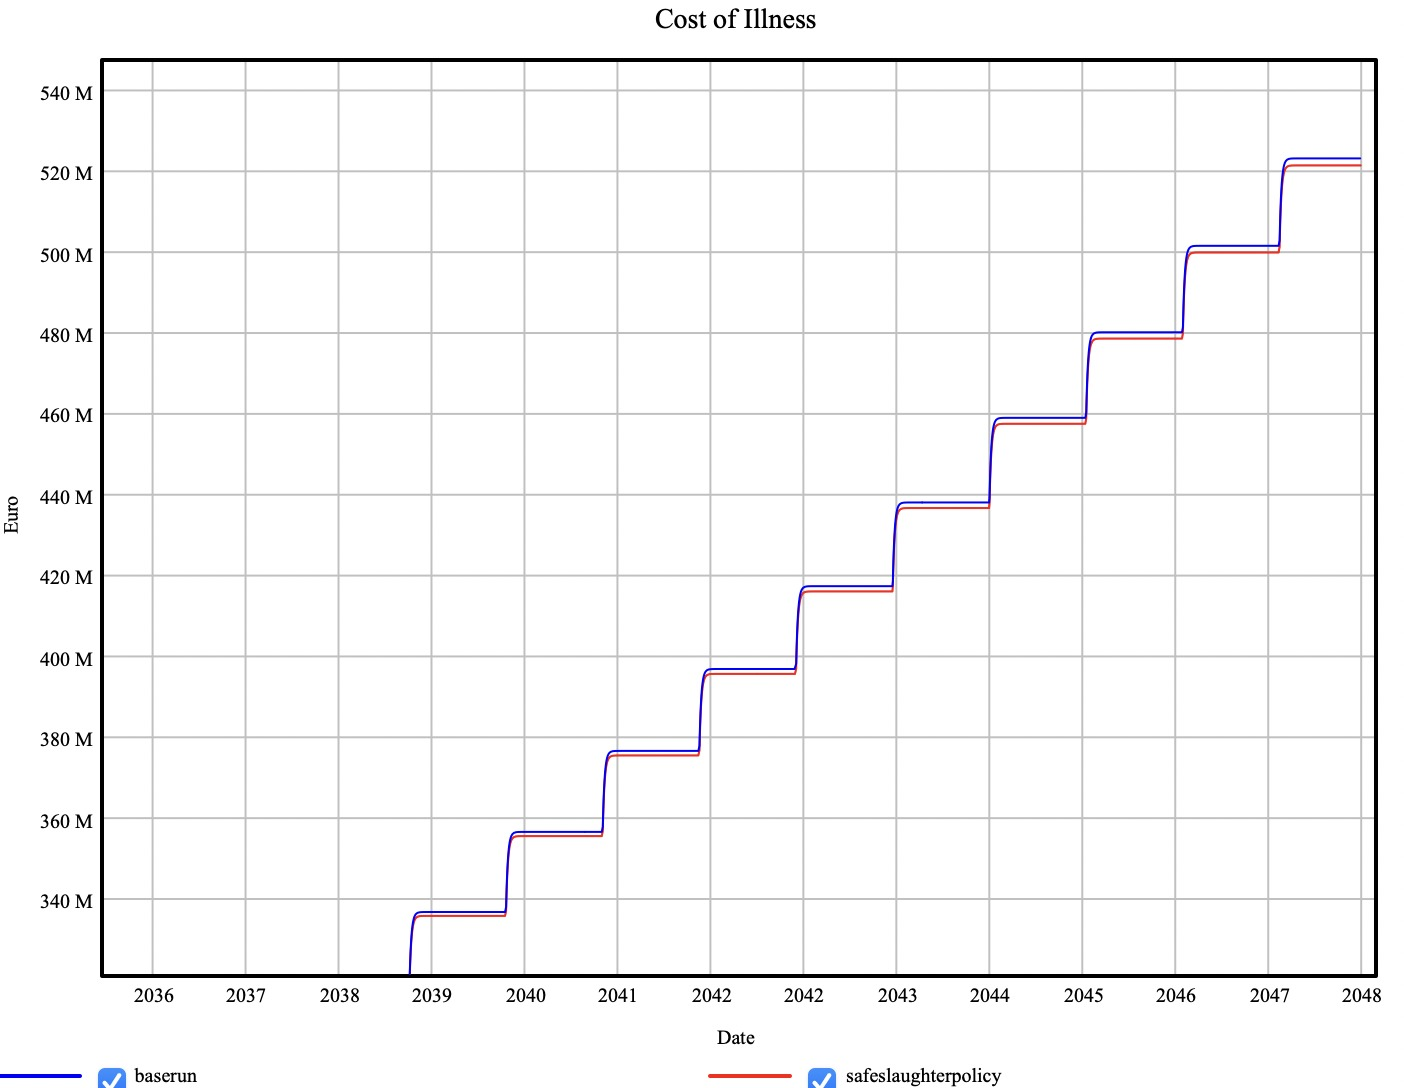
\includegraphics[width=1\textwidth]{images/p_coi.jpeg} 
        \caption{Cost of Illness in the Safe Slaughtering base run}
        \label{fig:p_coi}
    \end{minipage}\hfill
    \begin{minipage}{0.45\textwidth}
        \centering
        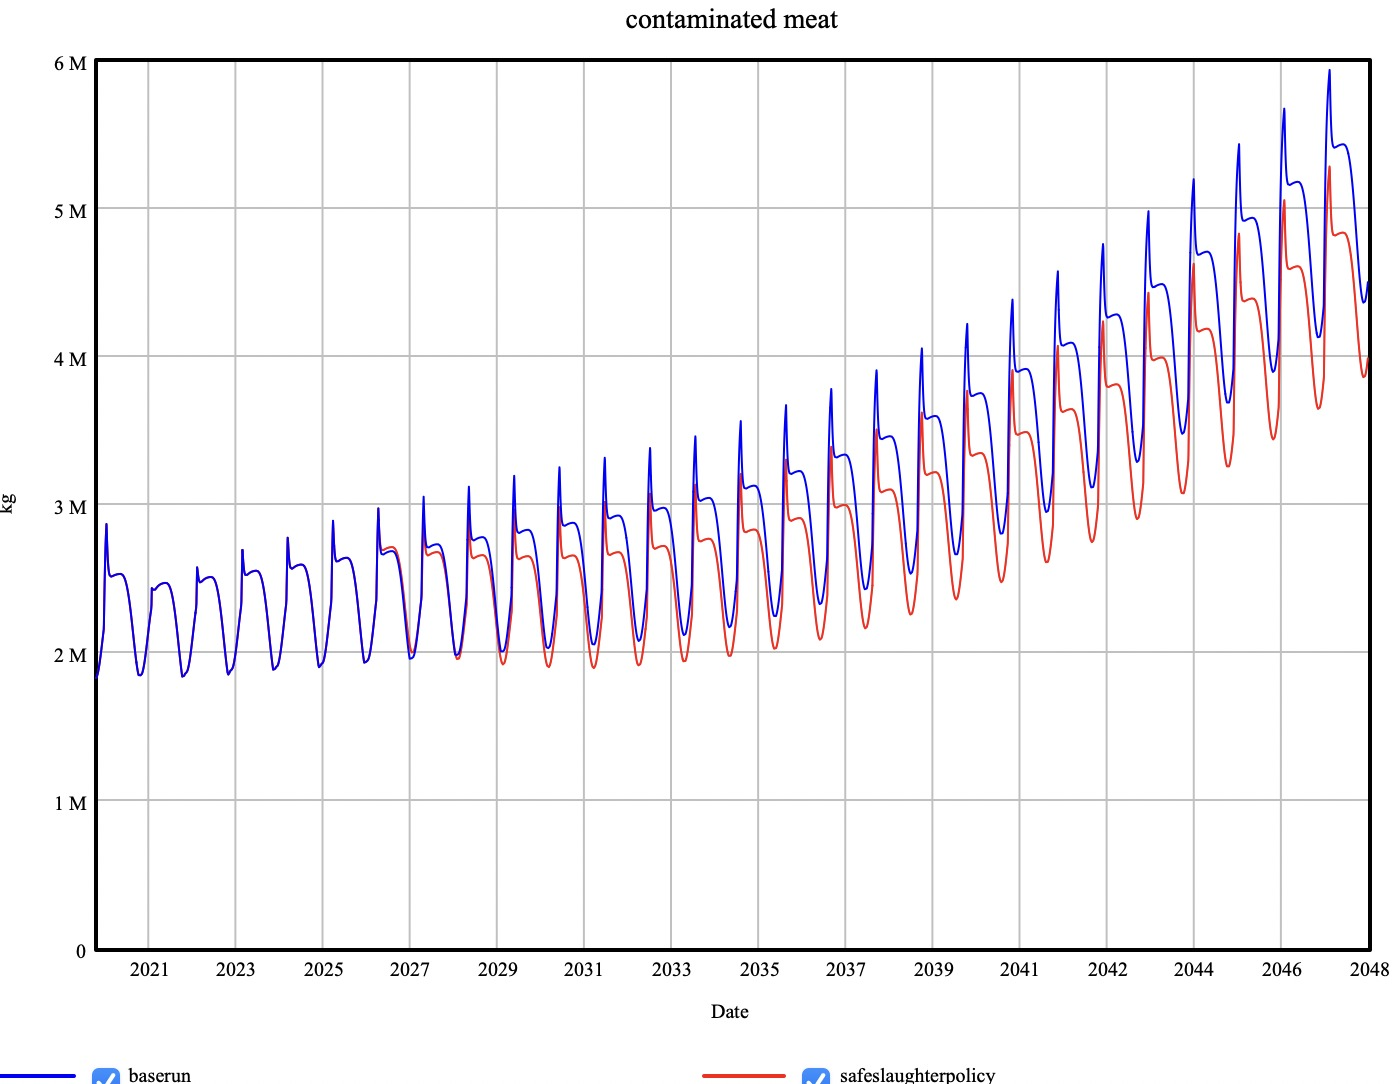
\includegraphics[width=1\textwidth]{images/p_meat.jpeg}
        \caption{Contaminated chicken meat in the Safe Slaughtering base run}
        \label{fig:p_meat}
    \end{minipage}
\end{figure} 

Model behaviour under this policy is reasonable. Once the food safety and handling policy goes into effect, the stock of contaminated meat decreases before slowly increasing again. This shows that it has an immediate effect, which stays over time but then continues growing. 

The odd spikes in Figure \ref{fig:p_meat} are similar to the ones as explained in section \ref{s:b_base}. 

Another policy implemented was the campaign to limit human exposure to flies, dubbed the No Fly Zone. This campaign would inform the Dutch population on how to minimise attractive environments for fly propagation. This policy reduces the rate of human exposure to infectious flies by 20\%. 

\begin{figure}[h!]
    \centering
    \begin{minipage}{0.45\textwidth}
        \centering
        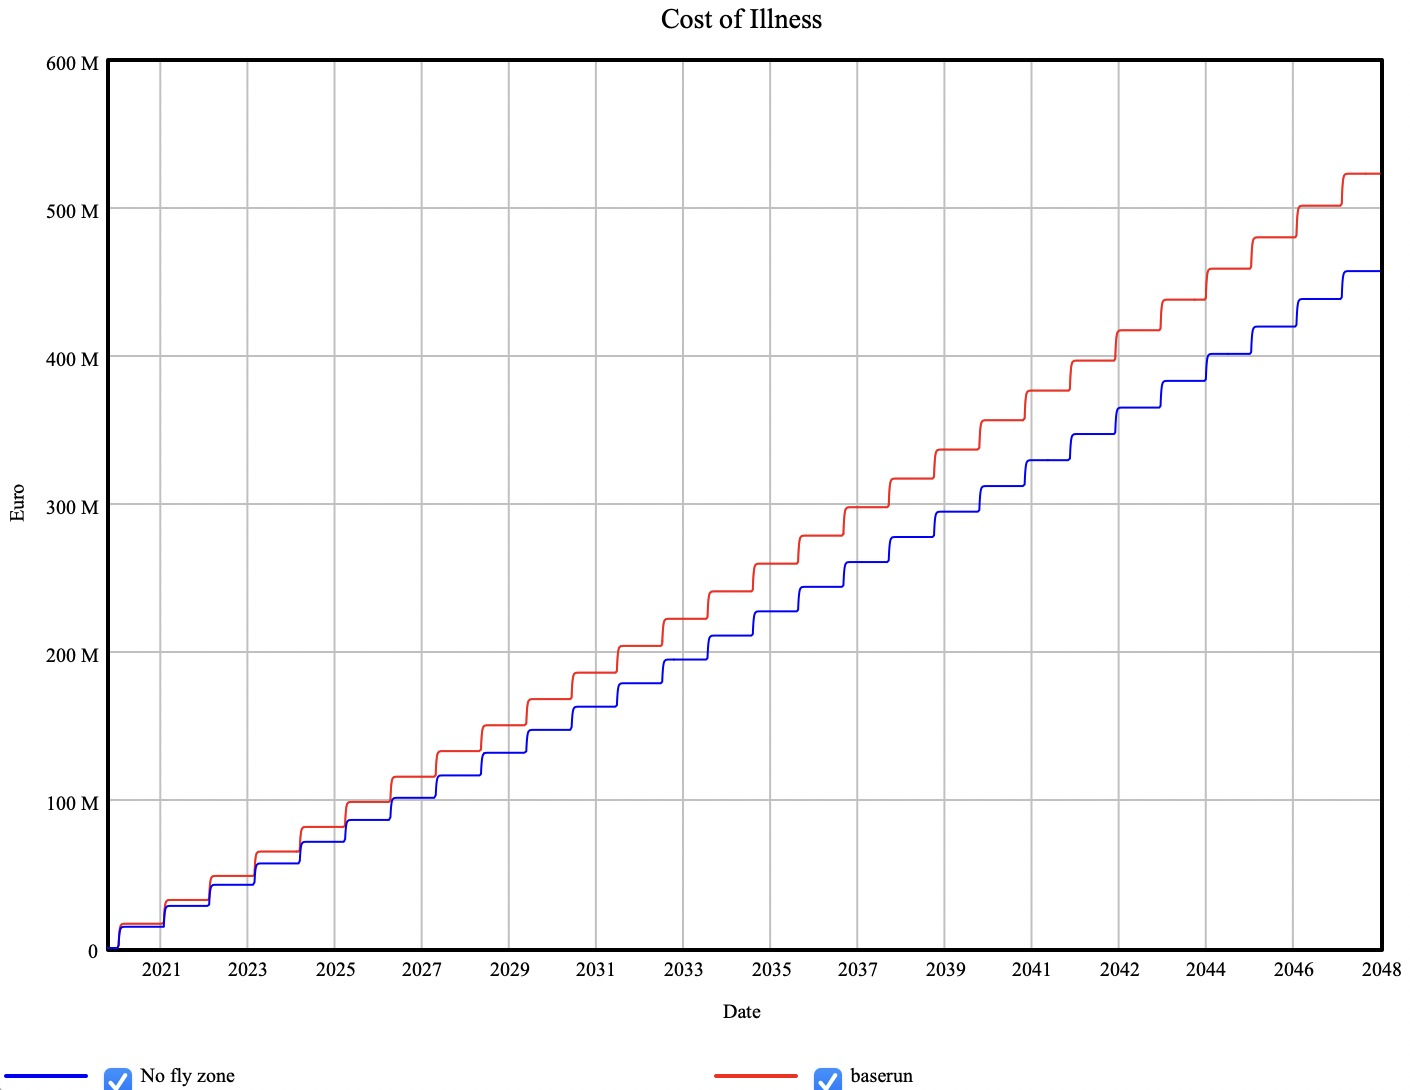
\includegraphics[width=1\textwidth]{images/p2_coi.jpeg} 
        \caption{Cost of Illness in the No Fly Zone base run}
        \label{fig:p2_coi}
    \end{minipage}\hfill
    \begin{minipage}{0.45\textwidth}
        \centering
        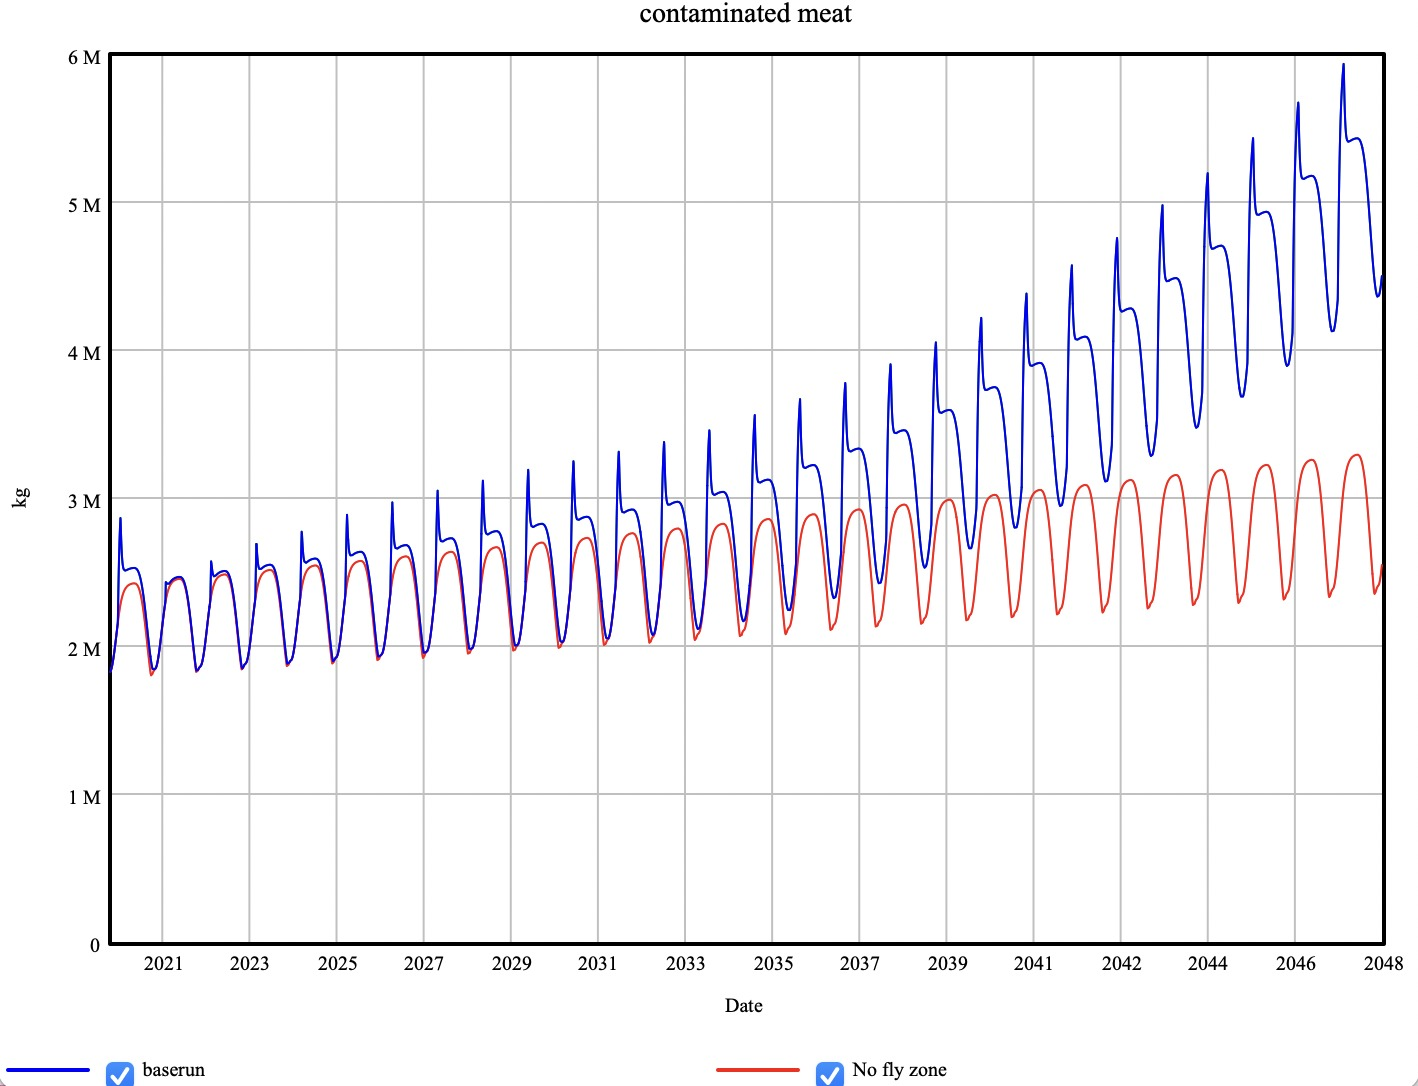
\includegraphics[width=1\textwidth]{images/p2_meat.jpeg}
        \caption{Contaminated chicken meat in the No Fly Zone base run}
        \label{fig:p2_meat}
    \end{minipage}
\end{figure} 

\begin{figure}[h]
\centering
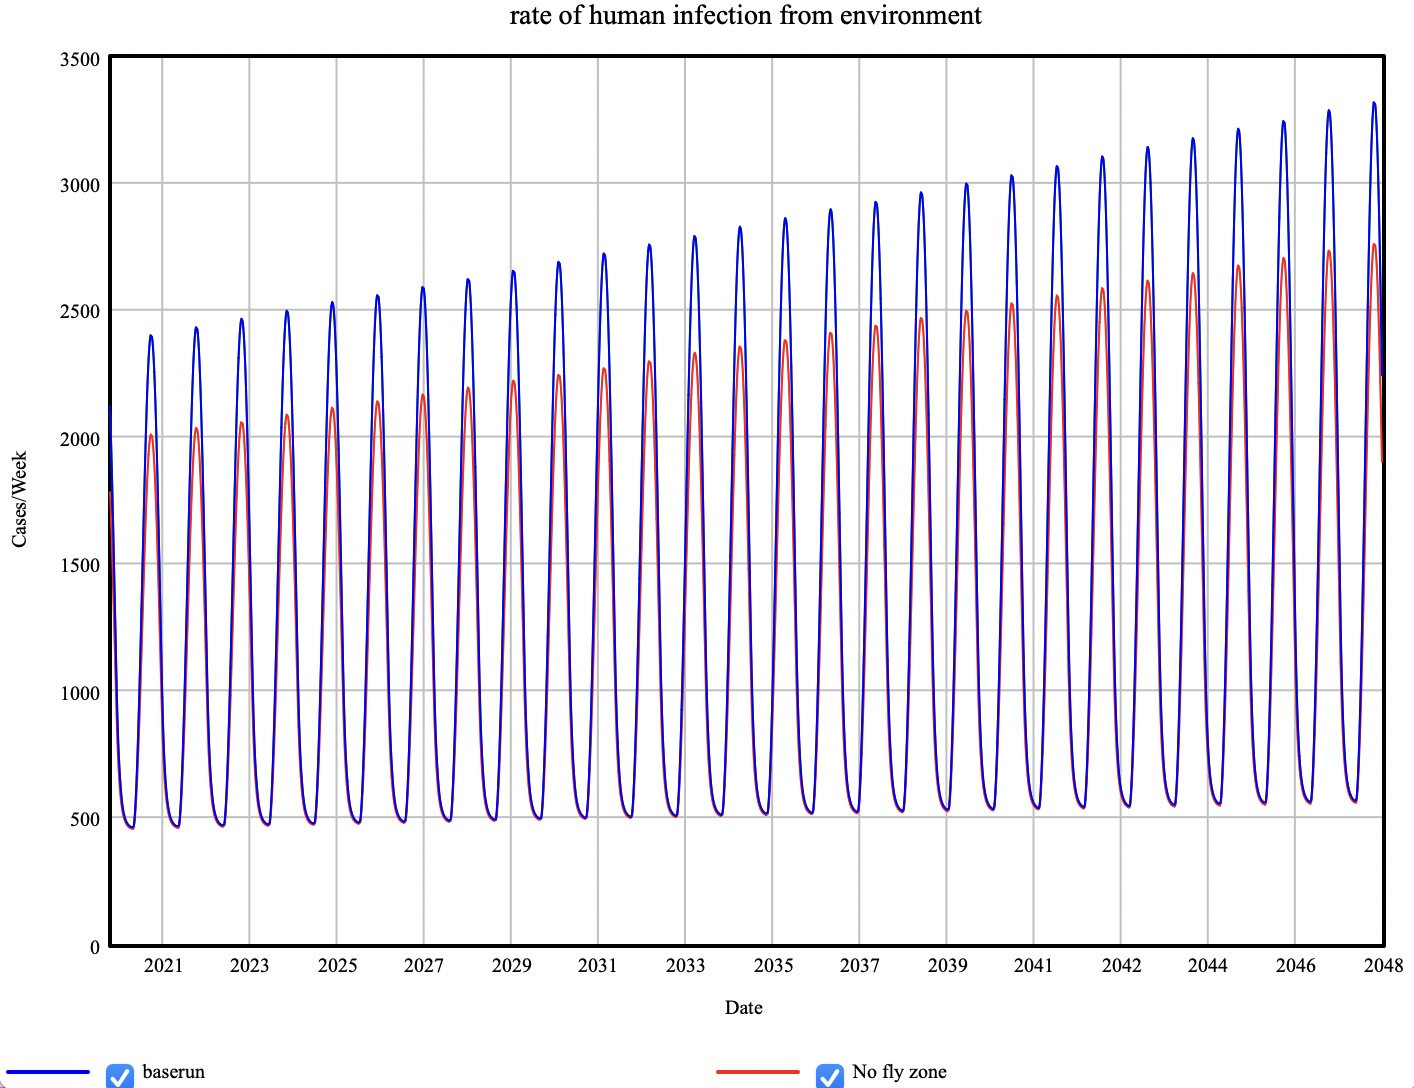
\includegraphics[width=0.45\textwidth]{images/p2_humanenvo.jpeg}
\caption{Human infections from the environment in the No Fly Zone base run }
\label{fig:p2_humanenvo}
\end{figure}

It can be seen in Figure \ref{fig:p2_meat} that the policy removes the strange peaks in the baserun. This is most likely due to the fact that the policy lowers the number of \textit{Campylobacter} cases, which mitigates the decrease of chicken meat consumption. This means that the threshold isn't met to trigger the meat consumption behaviour while the stock of contaminated meat decreases accordingly. 

Another fly related policy which was implemented is the the Pest Control policy. This Pest Control policy entails a policy that target the infectious flies and attempts to exterminate these fly populations in areas they would most likely be found, such as slaughterhouses and chicken farms.  

\begin{figure}[h!]
    \centering
    \begin{minipage}{0.45\textwidth}
        \centering
        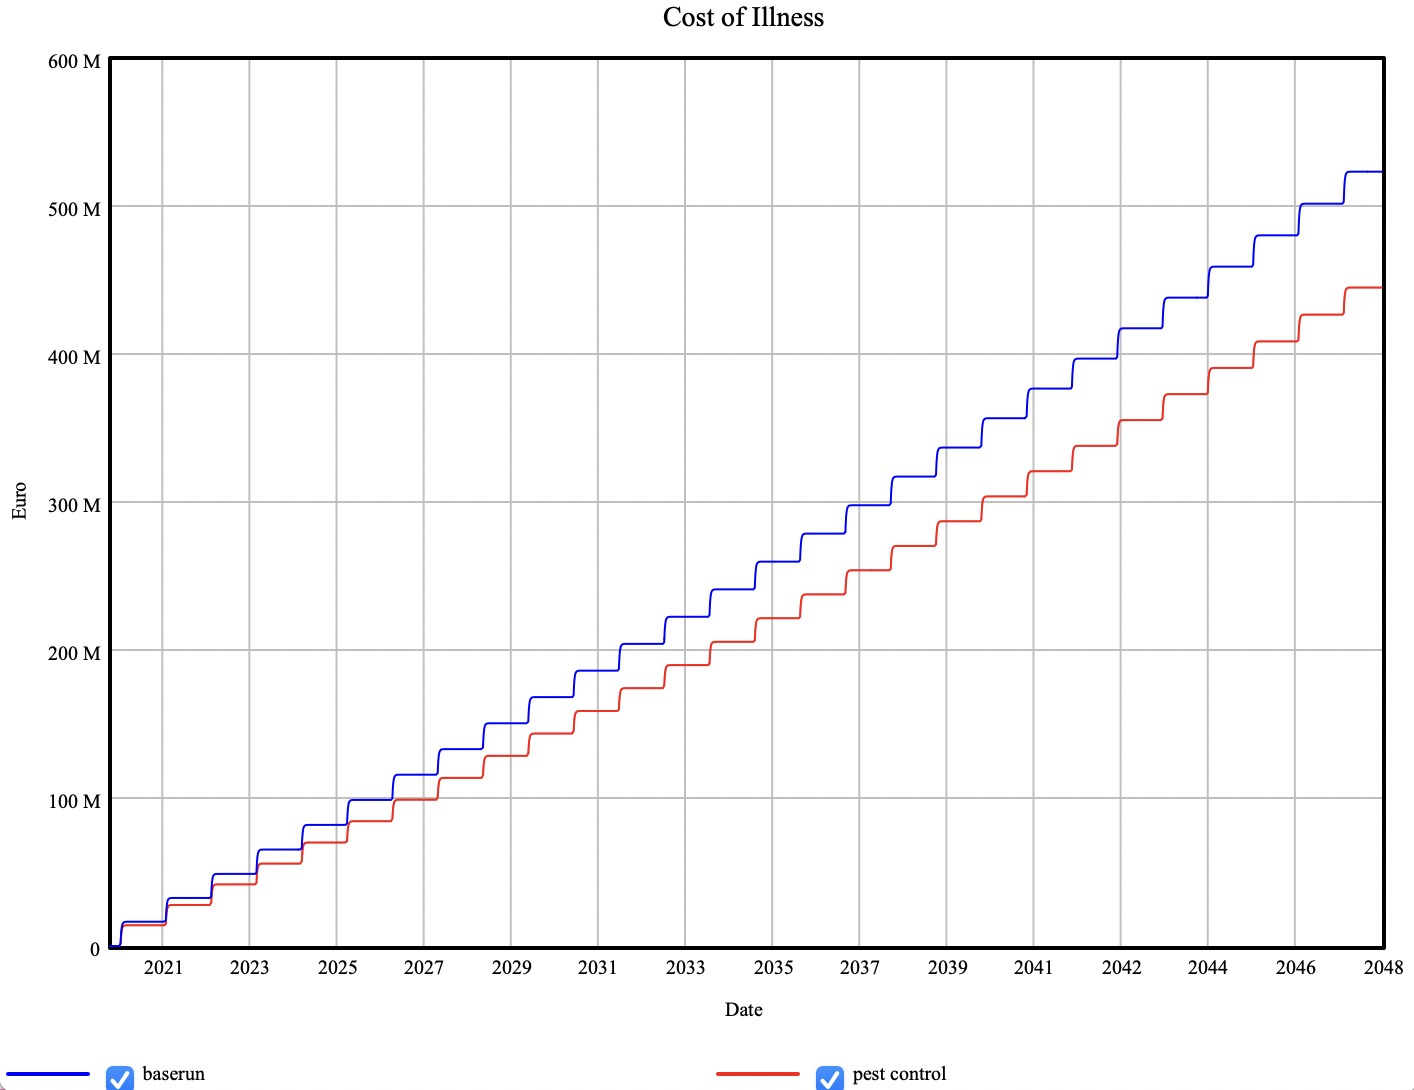
\includegraphics[width=1\textwidth]{images/p3_coi.jpeg} 
        \caption{Cost of Illness in the No Fly Zone base run}
        \label{fig:p3_coi}
    \end{minipage}\hfill
    \begin{minipage}{0.45\textwidth}
        \centering
        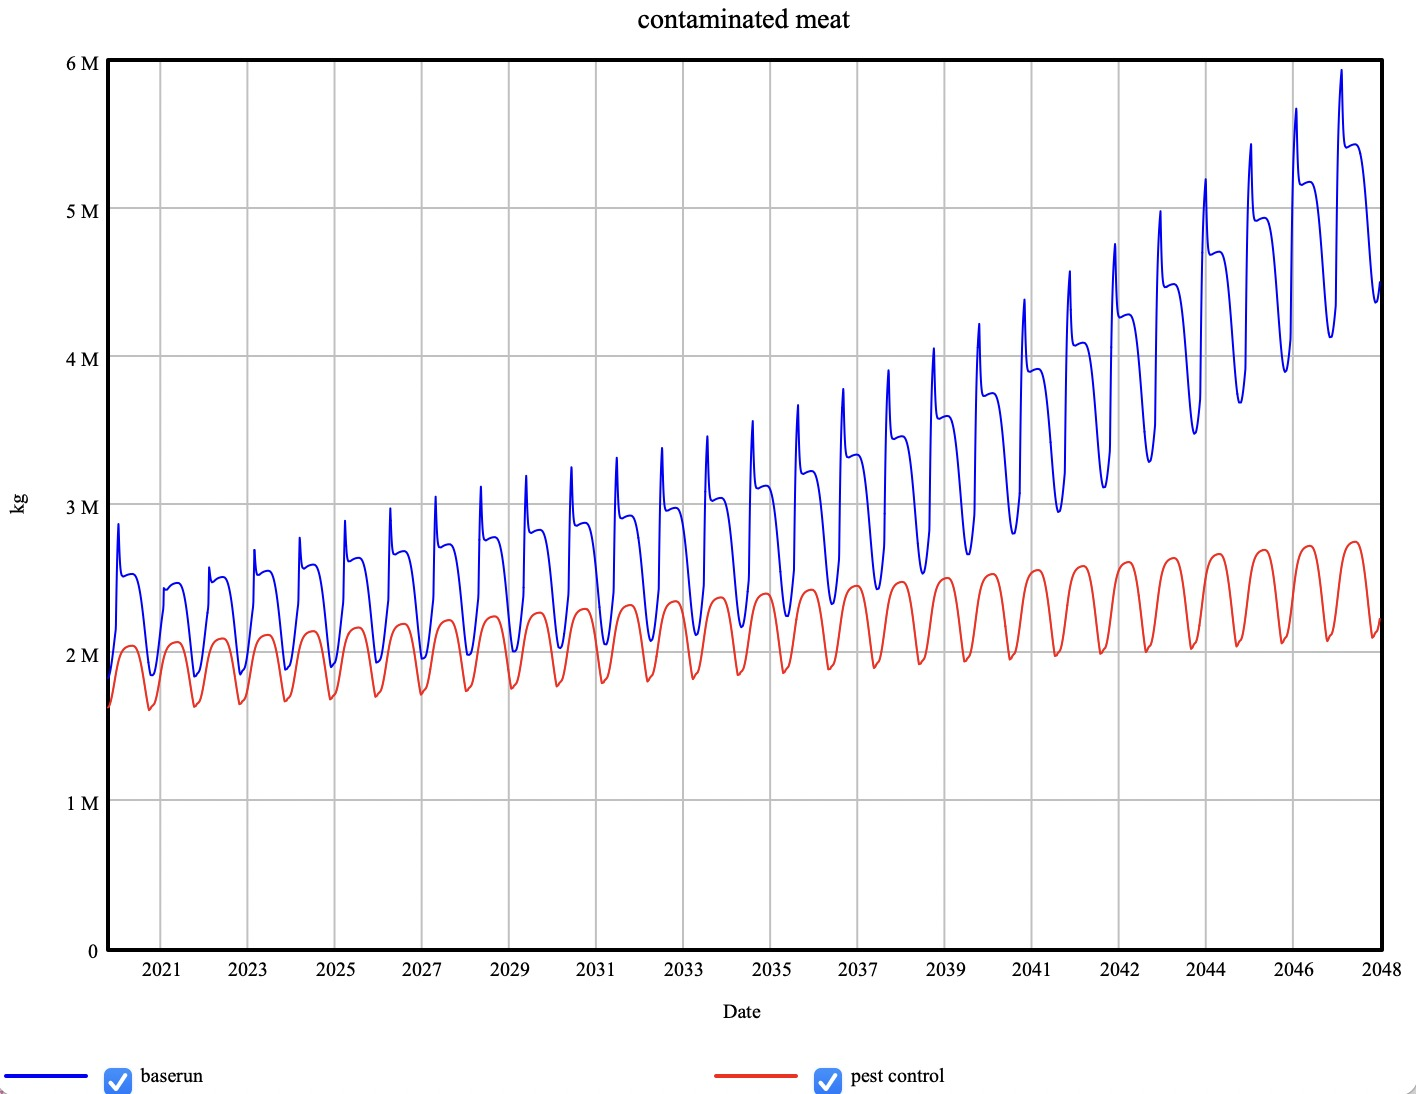
\includegraphics[width=1\textwidth]{images/p3_meat.jpeg}
        \caption{Contaminated chicken meat in the No Fly Zone base run}
        \label{fig:p3_meat}
    \end{minipage}
\end{figure} 

\begin{figure}[h!]
    \centering
    \begin{minipage}{0.45\textwidth}
        \centering
        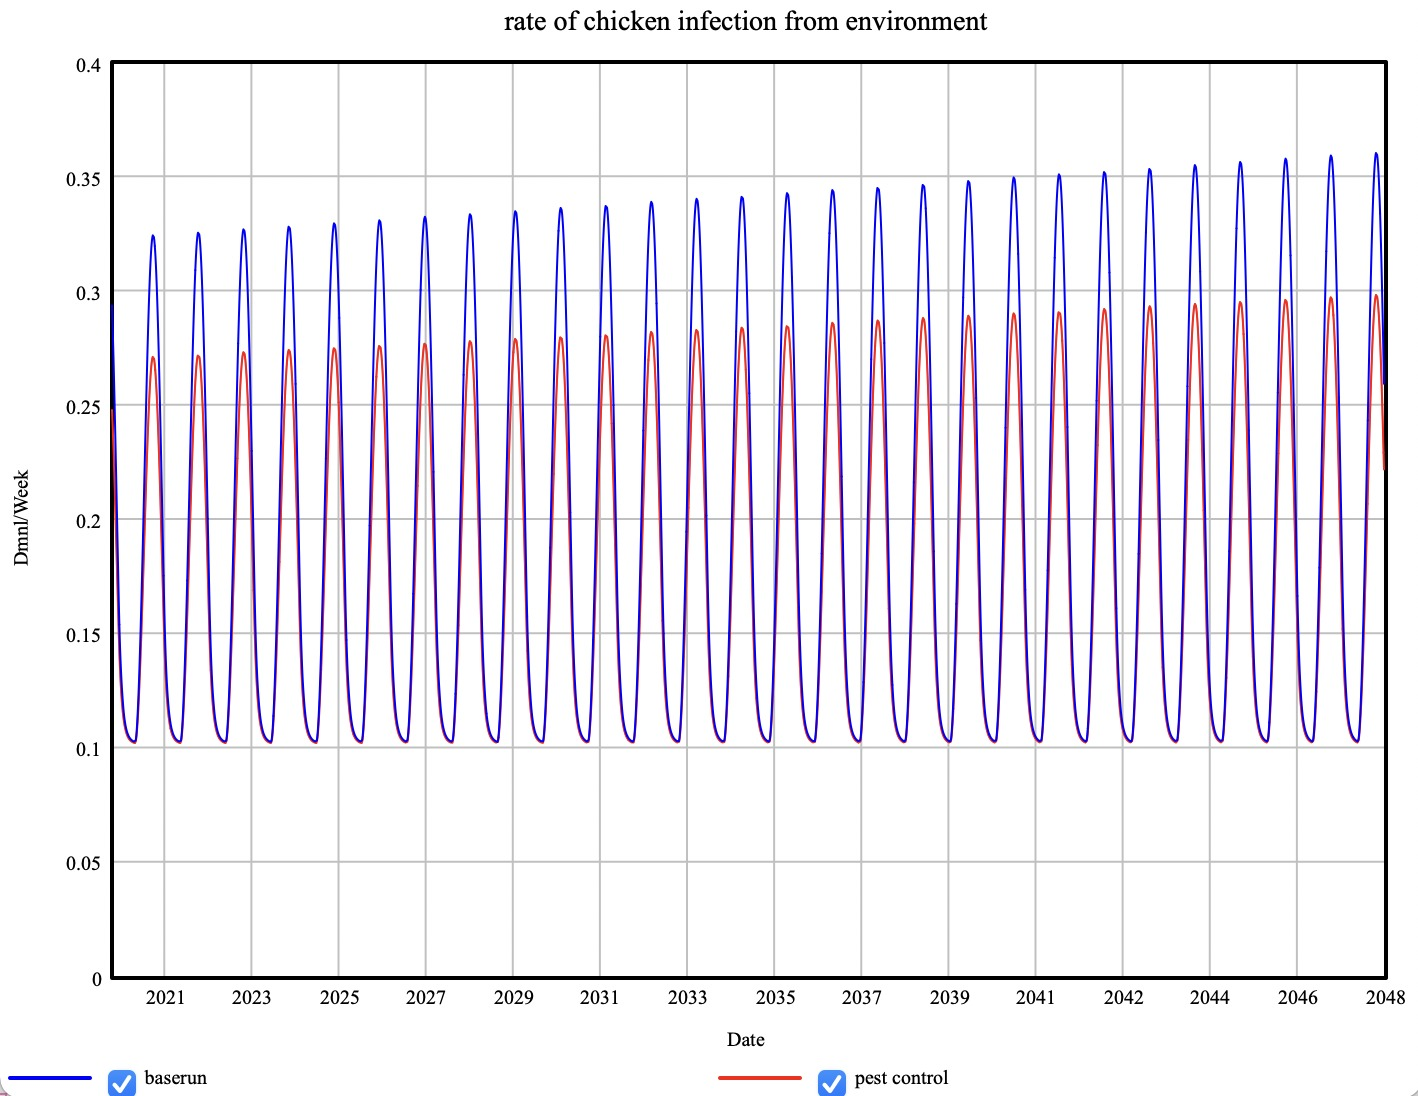
\includegraphics[width=1\textwidth]{images/p3_chicken.jpeg} 
        \caption{Chicken infections from the environment in the Pest Control base run}
        \label{fig:p3_chicken}
    \end{minipage}\hfill
    \begin{minipage}{0.45\textwidth}
        \centering
        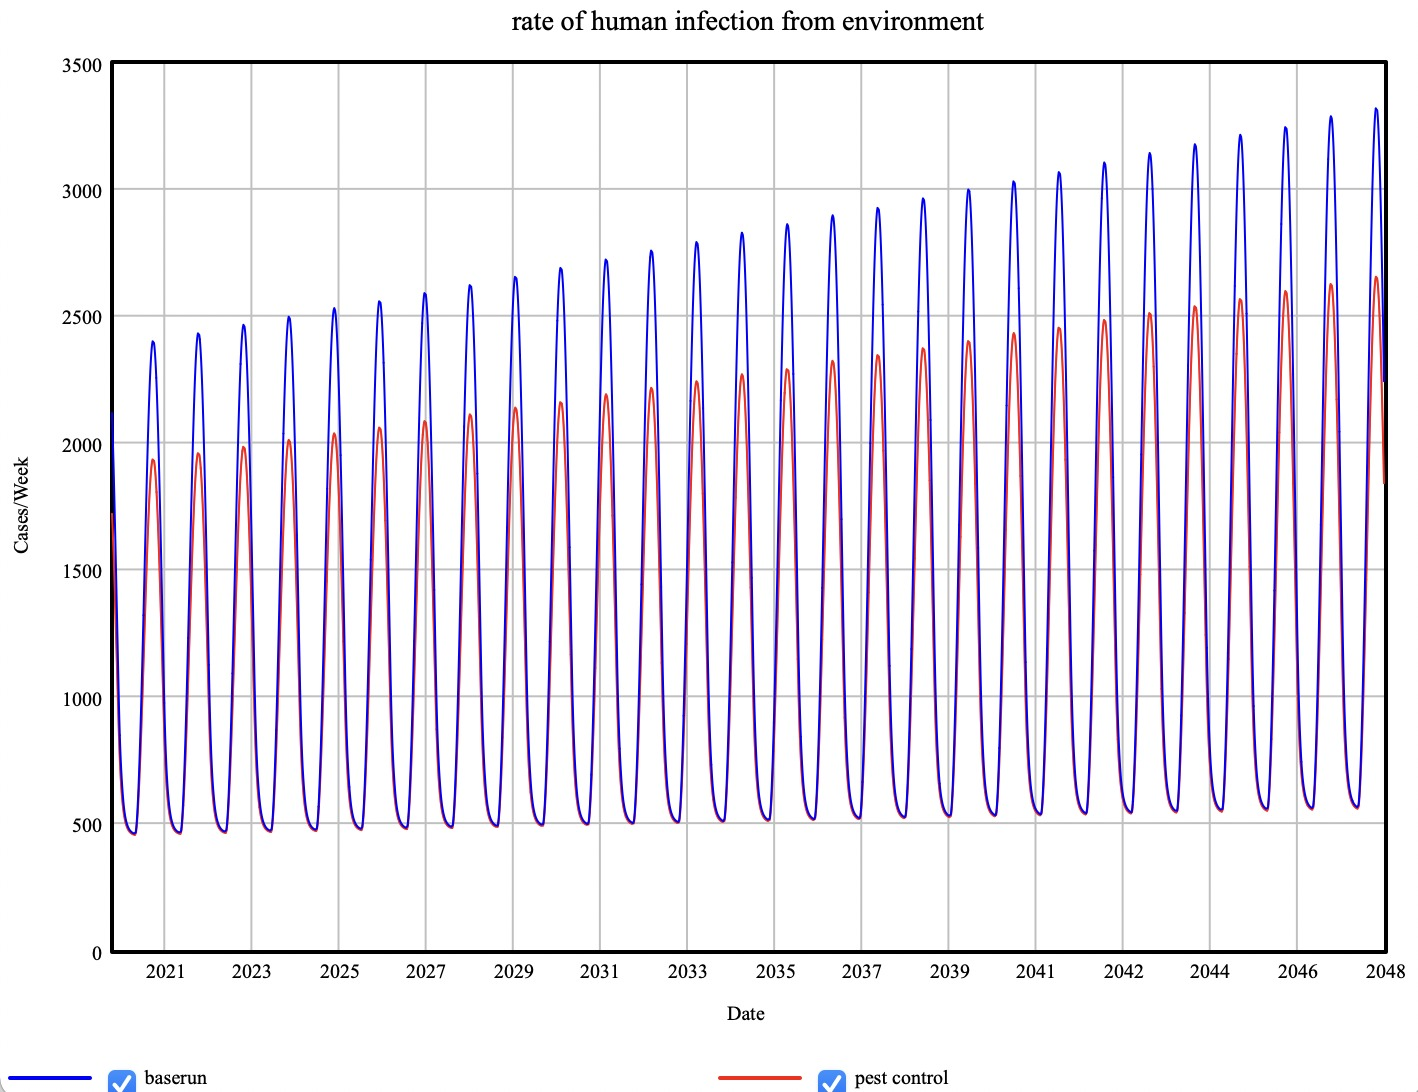
\includegraphics[width=1\textwidth]{images/p3_human.jpeg}
        \caption{Human infections from the environment in the Pest Control base run}
        \label{fig:p3_human}
    \end{minipage}
\end{figure} 

Two more policies regarding food were implemented, named food behaviour and preparation policies. Similar to the Safe Slaughtering policy, these policies go into effect when Cost of Illness reaches the 100 million threshold. These policies act on
\textit{consumption rate per person} and \textit{infections per kg of meat} respectively, by reducing these by 20\%.  

\begin{figure}[h!]
    \centering
    \begin{minipage}{0.45\textwidth}
        \centering
        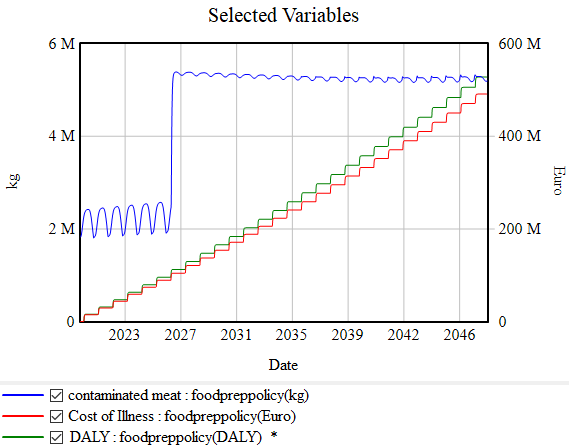
\includegraphics[width=1\textwidth]{images/foodbehaviourpolicy.png} 
        \caption{KPIs under food behaviour policy}
        \label{fig:foodbehav}
    \end{minipage}\hfill
    \begin{minipage}{0.45\textwidth}
        \centering
        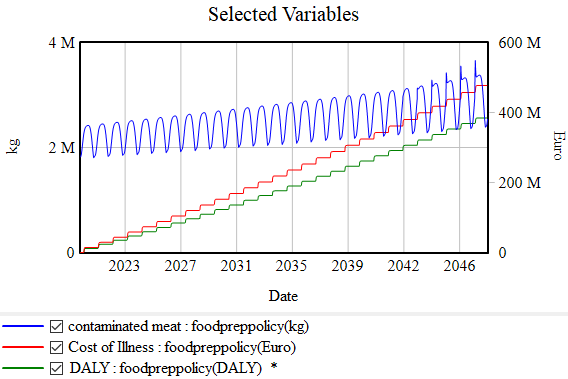
\includegraphics[width=1\textwidth]{images/foodpreparationpolicy.png}
        \caption{KPIs under food preparation policy}
        \label{fig:foodprep}
    \end{minipage}
\end{figure}

\fi

\subsection{Details on experiments}
\label{ch: detexp}
The policies employed in the model were tested against twelve scenarios, as detailed in Table \ref{tab:scenarios}. Scenarios 0, 1, 5 and 9 have the same values and are all baselines. The baseline simply contains a population increase that is also the medium increase, a temperature increase of 1.5 \degree c, a linear temperature change, and no rate of symptomatic cases modifier.

% Please add the following required packages to your document preamble:
% \usepackage{multirow}
\begin{table}[h!]
\caption{Scenarios under which the policies were tested for robustness}
\begin{tabular}{cl|lllll}
\hline
\multicolumn{1}{l}{}                                                           &                     &    & \multicolumn{4}{c}{Variable to change} \\ \cline{3-7} 
\multicolumn{2}{c|}{Test} &
  \multicolumn{1}{c}{\begin{tabular}[c]{@{}c@{}}Scenario\\ number\end{tabular}} &
  \multicolumn{1}{l}{\begin{tabular}[c]{@{}l@{}}Population \\ increase \\ by 2050\end{tabular}} &
  \multicolumn{1}{l}{\begin{tabular}[c]{@{}l@{}}Temperature \\ increase \\ by 2050\end{tabular}} &
  \begin{tabular}[c]{@{}l@{}}Temperature \\ switch\end{tabular} &
  \begin{tabular}[c]{@{}l@{}}Rate of \\ symptomatic \\ cases modifier\end{tabular} \\ \hline
\multicolumn{1}{l}{}                                                           & Baseline            & 0  & 1,94E+07     & 1.5     & 1    & 1      \\ \hline
\multirow{3}{*}{Population}                                                    & Medium increase     & 1  & 1.94E+07     & 1.5     & 1    & 1      \\
                                                                               & Large increase      & 2  & 2.16E+07     & 1.5     & 1    & 1      \\
                                                                               & Decrease            & 3  & 1.71E+07     & 1.5     & 1    & 1      \\ \hline
\multirow{3}{*}{\begin{tabular}[c]{@{}c@{}}Temperature \\ Change\end{tabular}} & 1 degree            & 4  & 1.94E+07     & 1       & 1    & 1      \\
                                                                               & 1.5 degree          & 5  & 19.4E+06     & 1.5     & 1    & 1      \\
                                                                               & 2 degree            & 6  & 19.4E+06     & 2       & 1    & 1      \\ \hline
\multirow{3}{*}{Seasonality}                                                   & No temp change      & 7  & 19.4E+06     & 1.5     & 0    & 1      \\
                                                                               & Fast temp change    & 8  & 19.4E+06     & 1.5     & 2    & 1      \\
                                                                               & Linear temp change  & 9  & 19.4E+06     & 1.5     & 1    & 1      \\ \hline
\multirow{2}{*}{\begin{tabular}[c]{@{}c@{}}Public \\ Health\end{tabular}}      & 10\% fewer symptoms & 10 & 19.4E+06     & 1.5     & 1    & 0.9    \\
                                                                               & 10\% more symptoms  & 11 & 19.4E+06     & 1.5     & 1    & 1.1    \\ \hline
\multicolumn{1}{l}{}                                                           & Worst case          & 12 & 2.16E+07     & 2       & 2    & 1.1   
\end{tabular}
\label{tab:scenarios}
\end{table}

%TC:endignore